\documentclass[11pt, parskip=half*,twoside=false]{scrbook}
\usepackage{todonotes}
\usepackage{natbib}
%\usepackage[utf8]{inputenc}
\usepackage[hidelinks]{hyperref}
\usepackage[UKenglish]{babel}
\usepackage[nottoc,notlot,notlof]{tocbibind}
\usepackage[UKenglish]{datetime}
\usepackage{graphicx}
\graphicspath{{./images/}}

\newdateformat{monthyear}{%
	\monthname[\THEMONTH] \THEYEAR}

% Commands required for using the Bath-Harvard citation standard
\newcommand*{\urlprefix}{Available from: }
\newcommand*{\urldateprefix}{Accessed }
\bibliographystyle{bathx}

% No indents in references
\setlength\bibhang{0pt}
% This package allows linebreaks in URLs, fixing a problem with long URLs in the References
\usepackage{xurl}

\RedeclareSectionCommand[
runin = true,
beforeskip = 0.5\baselineskip,
afterskip = -1em]
{paragraph}

\renewcaptionname{UKenglish}{\bibname}{References}             %Bibliography

% Set up acronyms
\usepackage[toc, nogroupskip, nonumberlist, nopostdot]{glossaries}
\makenoidxglossaries
\setacronymstyle{long-short}
\loadglsentries{gls_defns}

\usepackage[noabbrev]{cleveref}

%opening
\title{Low cost attentiveness detection systems}
\author{Thomas M. S. Smith}
\subtitle{A literature review and project plan submitted to the University of Bath in partial fulfilment of the requirements for the award of MSc in Robotics and Autonomous Engineering}
\publishers{Department of Electronic \& Electrical Engineering \\ University of Bath}
\monthyear

\begin{document}

\maketitle

\frontmatter

\chapter*{Declaration}

This literature review and project plan is submitted to The University of Bath in accordance with the requirements of the degree of Master of Science in Robotics and Autonomous Systems, in the Department of Electrical and Electronic Engineering. No portion of the work in this document has been submitted in support of an application for any other degree or qualification of this or any other university or institution of learning. Except where specifically acknowledged, it is the work of the author.

\vskip 2cm
\noindent\begin{tabular}{@{}p{0.5\textwidth}p{0.5\textwidth}@{}}
	\dotfill                         & \dotfill\\
	Thomas Smith              & Date\\
\end{tabular} 


\addchap{Abstract}
Aim for 150-300 words


\tableofcontents

\printnoidxglossary[sort=letter, title={List of Abbreviations}]

\chapter*{Acknowledgements}


\mainmatter


\chapter{Introduction} \label{ch:intro}
This chapter presents an introduction to the project and to this report. Present the motivation and background for the project, before laying out the structure of the report.

\section{Motivation} \label{sec:motive}

\paragraph{Notes}
\begin{itemize}
	\item Road traffic collision casualty numbers
	\item Driver inattention and distraction as contributor to road traffic collisions
	\item Increasing adoption of level 2 and 3 ADAS systems, still require full driver attention
	\item Possible application in level 4 and 5 systems
	\item Vital sign monitoring as part of attentiveness detection, and value of non-contact vital sign monitoring in healthcare settings
	\item Highlight opportunities for translation from healthcare to this application
	\item Briefly discuss challenges of transition (different environment, different subject status)
\end{itemize}

Driver inattention is one of the leading causes of \glspl{rtc} \citep{petridouHumanFactorsCausation2000,youngDriverDistraction2007,olsonDriverDistractionCommercial2009}. The increasing adoption of driving automation systems has the potential to improve road safety and reduce the incidence and severity of \glspl{rtc} \citep{favaroExaminingAccidentReports2017} but the introduction of such systems does present additional challenges for driver inattention. A number of collisions involving automated driving systems have been reported where the driver appears to have failed to provide the required level of supervision to the automated system, see for example \citep{ntsbCollisionSportUtility2019,ntsbCollisionCarOperating2019}. Existing methods of monitoring driver attentiveness in production vehicles, such as Tesla's monitoring of steering wheel torque, are easily defeated by a user and so do not provide sufficient protection. The large contribution to \glspl{rtc} made by driver inattention, coupled with the increasing adoption of automated driving systems, are the primary motivation for this work. A robust driver attentiveness monitoring system may reduce accidents in manual driving by encouraging drivers to, for example, rest when fatigued, and may also facilitate the wider and safer adoption of automated driving systems which will in turn reduce \gls{rtc} instances. 

A common approach for driver attentiveness monitoring is based on the measurement of driver vital signs, with \gls{ncvs} monitoring being particularly suited to the automotive environment. This presents an opportunity to benefit from and to contribute to advances in the field of healthcare in \gls{ncvs} monitoring. The continuous monitoring of the vital signs of the circulatory and respiratory systems is important for the monitoring and treating of many diseases in a variety settings, from the home to the ward. However it is impractical, and in some cases impossible, to use contact based measurements, motivating the development of various \gls{ncvs} monitoring approaches. 


\section{Report Structure} \label{sec:struct}
Brief overview of the document structure, as follows:
\begin{itemize}
	\item Literature review:
	\begin{itemize}
		\item Driver distraction and inattention:
		\begin{itemize}
			\item Why it matters
			\item Define taxonomy
			\item Present approaches from previous works:
			\begin{itemize}
				\item Driving behaviour measures
				\item Driver physiological measures (focus)
			\end{itemize}
			\item Detailed discussion of some key approaches:
			\begin{itemize}
				\item Relevance
				\item Strengths, weaknesses
				\item Reliability
				\item Accuracy
			\end{itemize}
		\end{itemize}
		\item Vital sign monitoring:
		\begin{itemize}
			\item Brief overview of major vital signs used in healthcare (personal and clinical settings)
			\item Brief overview of monitoring approaches used in personal and healthcare settings
			\item Focus on non-contact vital sign monitoring:
			\begin{itemize}
				\item Vision based (e.g. Lifelight)
				\item Radar based
				\item Other?
			\end{itemize}
		\end{itemize}
		\item Gaps and Opportunities
		\item Discussion/Analysis:
			\begin{itemize}
				\item Draw links between driver distraction/awareness and healthcare setting
				\item Highlight promising approaches
				\item Highlight challenges and gaps
				\item Conclude literature review
			\end{itemize}
		\end{itemize} 
	\item Project plan:
	\begin{itemize}
		\item Aims and objectives
		\item Specification
		\item Milestones and deliverables
	\end{itemize}
\end{itemize}


\chapter{Literature Review} \label{ch:litreview}
This chapter focusses on the literature review. Focus is driver inattention and distraction monitoring, and non-contact vital sign measurements.

\section{Driver distraction and inattention} \label{sec:distraction}

\subsection{Overview and definitions} \label{ssec:overview}
\paragraph{notes}
\begin{itemize}
	\item Highlight why driver attentiveness matters, introduce SAE autonomous vehicle levels, examples of when it goes wrong
	\item Discuss and define driver distraction and inattention
	\item Present taxonomy (either from \citep{reganDriverDistractionDriver2011} or specific to this work, prefer from source)
\end{itemize}

\paragraph{content}

\subsubsection{Automated driving systems}
As \glspl{ads} become more common and more advanced, the issue of driver inattention is likely to become even more critical. One particular area of concern is partially-autonomous vehicles, where the driver is still required to monitor and react to the environment while the \gls{ads} is performing certain driving tasks.  In \citep{J3016_201806} SAE International introduced a taxonomy and definitions for six levels of driving automation which is widely used in the discussion of autonomous vehicles. A summary of the six levels is shown in \cref{fig:av_levels}. These six levels of autonomy are based on four main factors which differentiate between whether the (human) driver or the automated system is responsible for certain tasks: 

\begin{enumerate}
	\item Who is performing primary driving actions (lateral and longitudinal control) 
	\item Who is detecting and responding to obstacles and events
	\item Who is the fallback should the automated system fail or reach an area outside of its operational design domain
	\item The extent and any limitations on the operational design domain\textemdash the environment(s) in which the automated system is designed to operate
\end{enumerate}

\begin{figure} 
	\centering
	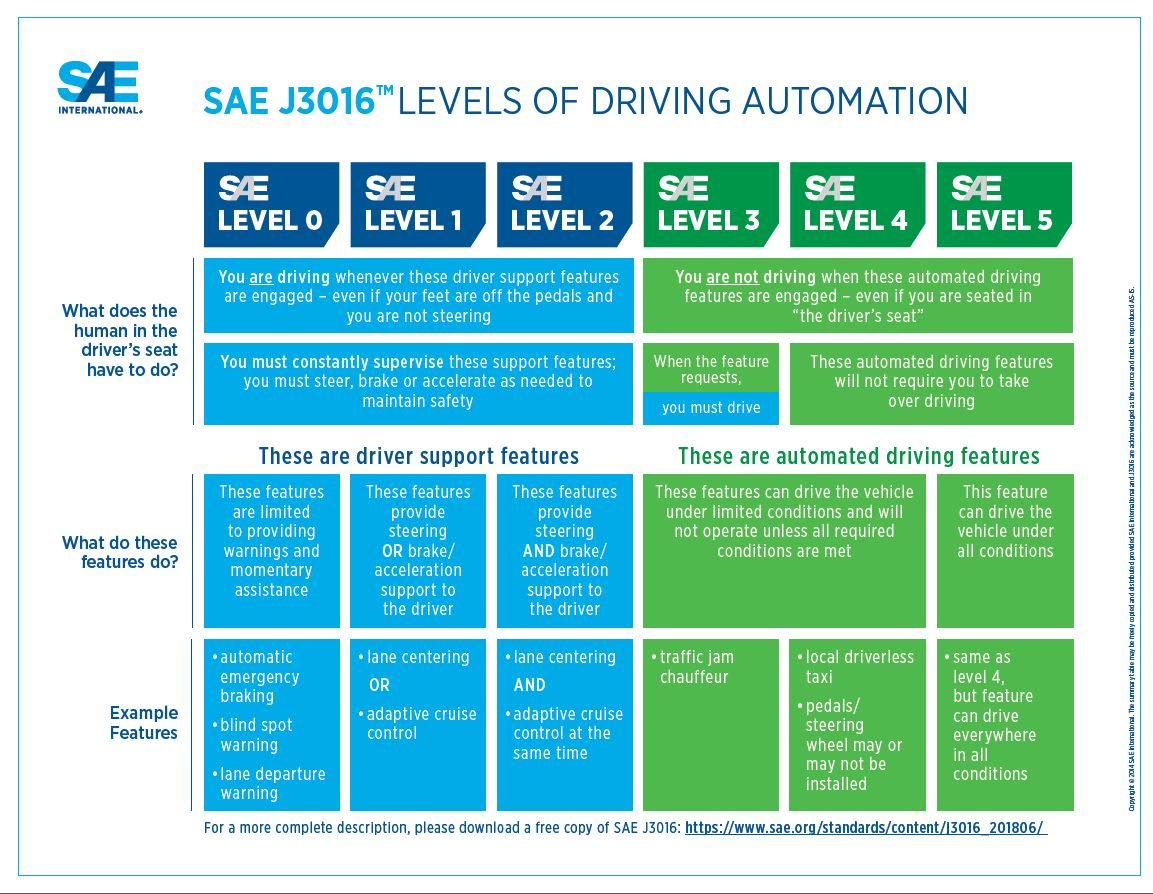
\includegraphics[width= \textwidth]{sae_av_levels} 
	\caption{Levels of driving automation. Reproduced AS-IS with permission from \citet{J3016_201806}}
	\label{fig:av_levels}
\end{figure}

A brief discussion of these levels of driving automation follows, highlighting the importance of driver attentiveness monitoring at the different levels of automation. 

SAE level 0 systems feature no driving automation. The human driver is always controlling the lateral (steering) and longitudinal (acceleration and braking) motion of the vehicle, and detecting and responding to obstacles and events during the driving task. There are exceptions for \gls{adas} such as automatic emergency braking, but these are not considered further here as they do not relate to the issue of driver attentiveness. Driver inattention and distraction is a concern in level 0 systems, with a review reporting driver inattention or distraction as a cause in approximately one quarter of \glspl{rtc} in the United States \citep{youngDriverDistraction2007}. A system with the capability to detect inattention or distraction could provide the driver with visual, audible or tactile alerts and warnings may increase driver attention or cause the driver to take a rest stop, and so reduce the likelihood of an \gls{rtc}.

In SAE levels 1 and 2 the human driver of the vehicle is always considered to be driving the vehicle, even if lateral and/or longitudinal control (steering and/or braking) is performed by the \gls{ads}. A level 1 system provides steering \emph{or} accelerator and brake support to the human driver, while a level 2 system can perform both tasks. The Tesla vehicles involved in the \glspl{rtc} in \cref{sec:motive} were SAE level 2 vehicles with the Tesla \gls{ads} system, `Autopilot' engaged. 

An SAE level 3 autonomous vehicle is capable of driving the vehicle under limited conditions, and the human is not considered to be the driver while the level 3 \gls{ads} is engaged. However the human driver must take back control of the driving task when requested to do so by the \gls{ads}. It is hopefully apparent that there are significant concerns and issues around driver distraction and inattention in level 1, 2 and 3 \gls{ads}, and these are areas where a low cost driver attentiveness monitoring system will offer benefits in safety and ....  \citet{teohWhatNameDrivers2020} report drivers consider many actions to be safe while a level 2 system is in operation, they're wrong, particularly bad for Autopilot. Prompt to remind drivers to pay attention, or disable the system where necessary etc...

Levels 4 and 5 can both be considered fully autonomous and the human driver is never expected or required to take control of the driving task. Level 4 is restricted to operate in limited circumstances, while level 5 automation can drive under all conditions. Driver attentiveness monitoring is not directly relevant to level 4 and 5 systems, however the closely related task of driver mood monitoring may be beneficial, allowing the \gls{ads} to tailor the vehicle ambience, driving route and style to the human occupants' current mood.

In addition to all of this, a driver monitoring system which includes monitoring of vital signs may provide valuable information to emergency response and accident investigation teams (driver is alive but deteriorating, driver was healthy before \gls{rtc} vs driver had heart attack before \gls{rtc}). 

\subsubsection{Driver inattention}
In this work we adopt the terminology of \citet{reganDriverDistractionDriver2011} when discussing driver inattention
In this work the term driver inattention is used according to the definition of \citet{reganDriverDistractionDriver2011} to mean `insufficient, or no attention, to activities critical for safe driving'. This inattention can stem from a number of different sources including fatigue and external distractions. The potential sources of inattention have implications for the design of an attentiveness monitoring system\textemdash an appropriate input signal detect fatigue induced inattention is likely to differ from a signal for distraction.  \citet{reganDriverDistractionDriver2011} identify five categories of driver inattention, resulting in the taxonomy presented in \cref{fig:taxonomy_inattention}. A brief discussion of these five categories is given here with the intention of identifying whether a category lends itself to monitoring via a driver attentiveness system. 

\begin{figure} 
	\centering
	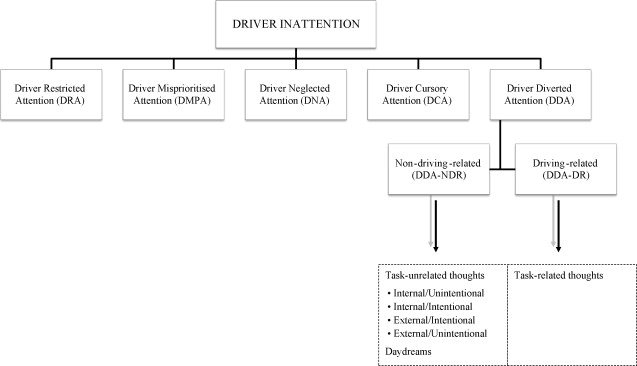
\includegraphics[width=\textwidth]{driver_inattention_taxonomy} 
	\caption{Taxonomy of driver inattention. Reproduced AS-IS with permission from \citep{reganDriverDistractionDriver2011}}
	\label{fig:taxonomy_inattention}
\end{figure}
\todo{REPRODUCE FIGURE, REMOVE DASHED BOXES}


\paragraph{\gls{dra}} inattention caused by biological factors (e.g. fatigue) and therefore can be monitored

\paragraph{\gls{dmpa}} incorrectly paying too much attention to one area of the driving task at the expense of a second equally or more important task. Probably can't be monitored but the consequences can be mitigated through \gls{adas} systems such as automatic emergency braking or blind-spot warnings

\paragraph{\gls{dna}}  TBC

\paragraph{\gls{dca}} cursory attention to elements of the driver task, for example a quick glance in the rear-view mirror without fully processing the scene. Probably can't be monitored but the consequences can be mitigated through \gls{adas} systems such as automatic emergency braking or blind-spot warnings

\paragraph{\gls{dda}} `The diversion of attention away from activities critical for safe driving towards a competing activity' \citep{reganDriverDistractionDriver2011}. This category encompasses driver distractions, whether related to the driving task, conversing with a passenger or on the telephone, or sending a text message, or watching a video etc...  

Some of these definitions are nuanced, and the authors themselves acknowledge that it is unlikely to be able to distinguish between some of the categories in practice. However the key points that are relevant to this work are that driver inattention can fall into a number of categories, with \gls{dra} and \gls{dda} being most relevant for a driver attentiveness monitoring system.

\gls{dra} and some of the \gls{dda} causes of inattention could be monitored by a driver attentiveness monitoring system, and this directs the remainder of this work.


\subsection{Approaches for monitoring inattention} \label{ssec:approaches}

\paragraph{notes}
Present existing methods, categorise as:
\begin{itemize}
	\item Driving behaviour measures:
	\begin{itemize}
		\item Driving input measures (steering, brakes, accelerator)
		\item Lane-keeping
		\item Spacing to surrounding vehicles
	\end{itemize}
	\item Driver physiological measures:
	\begin{itemize}
		\item Heart rate
		\item Eye motion tracking
		\item Vision based systems
		\item Head motion tracking
		\item Facial expressions
	\end{itemize}
	\item Discuss methods which combine measures
	\item Driver models (Kalman Filter of the driver?)
\end{itemize}


\paragraph{content}

\todo{Present summary diagram similar to fig. 3 of \citep{koesdwiadyRecentTrendsDriver2017}}

A number of approaches for driver attentiveness monitoring have been proposed in the literature, using a variety of measured signals to detect the different forms of driver inattention, \gls{dra} and \gls{dda}, introduced previously. Due to the different causes and symptoms of \gls{dra} and \gls{dda} some approaches are better suited to detecting one or the other. Monitoring approaches can either be categorised according to the form(s) of driver inattention they are best suited to monitoring or according the measures that are used to assess attentiveness. In this section relevant literature is identified and discussed according to the measures used, as this is more useful because..... A taxonomy for all the measures considered in this work is shown in \cref{fig:taxonomy_measures}



\begin{figure} 
	\centering
	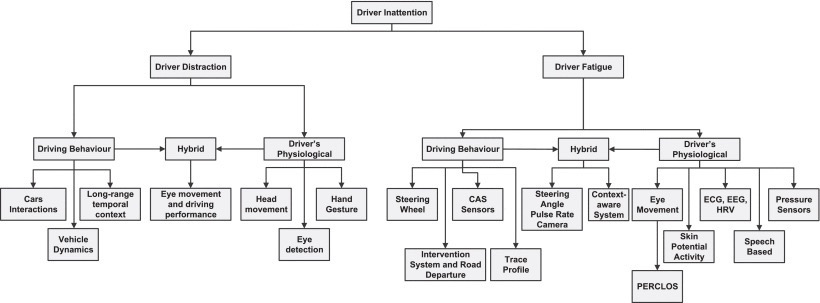
\includegraphics[width=\textwidth]{inattention_inputs_taxonomy} 
	\caption{Taxonomy of driver inattention measures}
	\label{fig:taxonomy_measures}
\end{figure}
\todo{REPRODUCE FIGURE TO REFLECT CONTENTS OF THIS WORK}


Consider the following works:
\begin{itemize}
 	\item \citet{wollmerOnlineDriverDistraction2011} Driving behaviour, \gls{lstm} tracking, head movement
	\item \citet{liangHybridBayesianNetwork2014} \gls{dbn} for driving behaviour and eye movement
	\item \citet{kurianDrowsinessDetectionUsing2014a} \gls{ppg} for fatigue detection
	\item \citet{zhangAutomatedDetectionDriver2014} Various entropy and complexity measures applied to \gls{eeg}, \gls{emg} and \gls{eog} signals
	\item \citet{tsuchiyaHeartbeatDetectionTechnology2020} heart rate detection via 24~GHz radar
	\item \citet{jungDriverFatigueDrowsiness2014} \gls{hrv} measurement via \gls{ecg} on steering wheel to monitor fatigue
	\item \citet{aksjonovDetectionEvaluationDriver2019} Fuzzy expert model for driver distraction detection
	\item \citet{liDetectionDriverDrowsiness2013} Fatigue detection from \gls{svm} applied to \gls{hrv} measured using \gls{ppg} 
	\item \citet{yuDriverDrowsinessDetection2019} vision based \gls{cnn} detection of fatigue
	\item \citet{gaoEEGBasedSpatioTemporal2019} \gls{eeg} based \gls{cnn}
	\item \citet{crayeMultiModalDriverFatigue2016} multi-modal detection of fatigue
	\item \citet{duaAutoRateHowAttentive2019}  A five rating scale of driver attentiveness based on \gls{cnn} and \gls{gru}
	\item \citet{greeleyDetectingFatigueVoice2006} Voice audio and speech recognition to detect fatigue
	\item \citet{fuDynamicDriverFatigue2016} \gls{hmm} applied to biological signals for fatigue detection
	\item \citet{dingInattentiveDrivingBehavior2019} \gls{fmcw} radar used to detect driver head movements for inattention detection
	\item \citet{liOnlineDetectionDriver2017} Steering wheel angles for driver fatigue detection
	\item \citet{zhouPredictingDriverFatigue2021} Explainable fatigue prediction, need to read in more detail
	
\end{itemize}




\paragraph{\citep{koesdwiadyRecentTrendsDriver2017}} A high-level survey of driver monitoring systems. It doesn't seem great but probably provides some good references to follow up on. Discusses types of driver inattention which is useful. Introduces a taxonomy of driver distraction monitoring sources which is probably worth exploring. Main sources of driver distraction detection:
\begin{itemize}
	\item Driving behaviour measures, including LSTM tracking head movement \citep{wollmerOnlineDriverDistraction2011}
	\item Physiological measures of driver (all vision based in this paper)
	\item Hybrid methods (driving behaviour and physiological measures)
\end{itemize}

Use of Dynamic Bayesian Networks to detect distraction via driving behaviour and eye movement \citep{liangHybridBayesianNetwork2014}

Main sources of driver fatigue detection:
\begin{itemize}
	\item Driving behaviour measures
	\item Physioological measures:
	\begin{itemize}
		\item Eye and face movement
		\item Speech
		\item PERCLOS (percent of eye closure)
		\item Skin \citep{kurianDrowsinessDetectionUsing2014a}
		\item Biological signals \citep{zhangAutomatedDetectionDriver2014}
	\end{itemize}
\end{itemize}

\paragraph{\citep{reganDriverDistractionDriver2011}} Introduces definitions and taxonomy for driver distraction and driver inattention (distinguishing between the two).

Driver inattention is defined as `insufficient, or no attention, to activities critical for safe driving'. This is a good reference with good taxonomy etc.

\paragraph{\citep{tsuchiyaHeartbeatDetectionTechnology2020}} 24GHz microwave Doppler radar based heart rate detection. Sensor is placed in seat back to avoid interference from arm motions  Vibrations (e.g. from driving) cause noise to be superimposed over the sensor signal reducing the SNR (signal to noise ratio). The authors introduce an algorithm to cope with this. 

Electrodes on steering wheels don't work if driver's hands are not on the wheel or the sensor, camera based systems raise concerns of intrusion / privacy. 

Electrocardiogram: peaks of electrical activity are called P,Q,R,S, and T-waves. Interval between two consecutive R peaks is heartbeat interval (R-R interval, RRI). A heartbeat generates a small displacement of the body surface which is detected by radar system. However  respiration and body movements fal in the same band, making it difficult to extract heartbeat.

Algorithm: Band-pass filter (BPF) -> short-time Fourier transform with Hamming window -> spectrum integration -> BPF -> peak detection

The approach is a very 'engineered' one, with a complex(?) algorithm. 

Experimental evaluation via in-car testing with ECG as reference sensor. Improved accuracy during driving compared to previous method but still poor equivalence to ECG reference sensor.

\paragraph{\citep{jungDriverFatigueDrowsiness2014}} Electrocardigram (ECG) sensor embedded in steering wheel. Sample ECG signals at 100 Hz. Driver state assessed by evaluating heart rate variability (HRV), the variation of the time interval between heart beats. HRV can be used to evaluate the autonomic nervous system (ANS) status and can indicate normal, fatigued and drowsy states. HRV analysis methods can be in the time domain or the frequency domain. Time domain HRV is based on beat-to-beat intervals, frequency based HRV is by measuring the power spectral density (PSD) using parametric fast Fourier transforms.

System was tested on two test subjects over a two hour driving test. results?

\paragraph{\citep{sikanderDriverFatigueDetection2019}} Fatigue detection methods are implemented as either: bio-mathematical models, rule based, or machine learning models. Remember that fatigue is only one of the causes of driver inattention.  A good reference and source of references for fatigue related approaches.

\begin{itemize}
	\item Bio-mathematical models are more relevant for workload management tasks (aircrew rotas, driver schedules etc.)
	\item Rule based models (like expert systems) include Fuzzy Inference Systems, e.g. \citep{aksjonovDetectionEvaluationDriver2019}
	\item Machine learning based implementations such as Artificial Neural Networks (ANN) or Support Vector Machines (SVM). Lots of references to consider....
	\begin{itemize}
		\item \citet{liDetectionDriverDrowsiness2013} use SVM classifier on PPG (photoplethysmography) derived HRV (heart rate variability)
		\item Vision based CNN approaches \citep{yuDriverDrowsinessDetection2019} and EEG based CNN approaches \citep{gaoEEGBasedSpatioTemporal2019}
	\end{itemize}
\end{itemize}

Figure 2 in Section \textsc{V} is a very good way of representing / summarising the approaches taken in previous works.

Separate methods from input sources.  Method exanples are:
\begin{itemize}
	\item Bio-mathematical
	\item Rule based
	\item Machine learning
\end{itemize}

Example signal sources are:
\begin{itemize}
	\item Driving behaviours (steering behaviour, lane keeping, driving time)
	\item Driver physiological measures (heart signal, brain signal, PERCLOS, eye tracking, posture)
	\item Hybrids
\end{itemize}

'rPPG is less explored for driver fatigue detection'


\subsection{Analysis}
Use preceding sub-section as input to discuss:
\begin{itemize}
	\item Trends
	\item Weaknesses
	\item Gaps
	\item Issues
\end{itemize}


\section{Vital sign monitoring}

\paragraph{\citep{singhMultiResidentNonContactVital2021}} Review paper of multi-resident non-contact vital sign monitoring using radar.

Applications in health care including infant monitoring, telehealth, sleep monitoring, skin allergies and burn cases.  Different none contact methods include:
\begin{itemize}
	\item Optical vibro-cardigraphy
	\item audio
	\item thermal imaging
	\item RGB camera
	\item ultrasound radar2
	\item microwave radar
\end{itemize}

Figure 2 in the paper gives a simple representation of a doppler radar based system. The original paper on noninvasive microwave measurement of respiration is  \citep{linNoninvasiveMicrowaveMeasurement1975}. The basic principle of measurement is based on Doppler shift caused by movement of the subject's chest wall.  Two most commonly used radar topologies are \gls{cw} (including \gls{fmcw}) and \gls{uwb}. Advantages and disadvantages are discussed in the paper (probably good to include). Table 1 in particular is a nice summary. Discusses radar front end architectures - heterodyne vs homodyne, single vs quadrature channel.

Section D gives a good overview of how radar \gls{ncvs} works. One way to increase SNR is by increasing transmission power but there are limits as this can lead to damage to tissue / harm to health etc. FInd a source for guidelines / standards / regulations / legislation?

Increasing frequency reduces wavelength and increases the sensitivity to small displacements. mmWave region corresponds to frequencies between 30~GHz to 300~GHz.  Higher frequencies have numerous advantages:
\begin{itemize}
	\item Improved range resolution
	\item Reduced device form factor
	\item Improved directionality and therefore increased range
\end{itemize}

Is attenuation an issue around the 60 GHz range?

Figure 5 gives an excellent view of the frequencies investigated for \gls{ncvs} in previous works


Discuss vital sign monitoring in a healthcare setting (personal and clinical), with a view to potential cross-overs between driver distraction and inattention monitoring and vital sign monitoring (in both directions).
\subsection{Vital signs}
Briefly introduce and define the key vital signs used in healthcare settings (`textbook' definitions)
\subsection{Approaches for monitoring vital signs}
Brief overview of existing vital sign monitoring approaches:
\begin{itemize}
	\item Contact based (very brief)
	\item Non-contact based (focus)
	\begin{itemize}
		\item Vision based
		\item Radar based
		\item Other?
	\end{itemize}
\end{itemize}

\section{Gaps and opportunities}
Highlight gaps in existing works, along with any opportunities presented by these gaps or by extending or combining existing approaches

\section{Discussion}
Draw links between driver distraction/awareness and healthcare setting,highlight promising approaches and directions, and existing challenges to overcome. Draw the literature review to a close by summarising review and findings. 


\chapter{Project Plan}
This chapter presents the objectives, specification and plan for the project

\section{Aims and objectives}
\begin{itemize}
	\item Aims as high-level intentions for the project (e.g. the proof of concept design, development and testing of an attentiveness monitoring system with possible applications in automotive and healthcare settings). Show clear connection to literature review. 
	\item Overview of the objectives, probably list form. Include stretch goals.
\end{itemize}

\section{Specification}
\begin{itemize}
	\item What will the proposed system do?
	\item How will it do it?
	\item Hardware/software deliverables
\end{itemize}

\section{Milestones and deliverables}
\begin{itemize}
	\item Gantt chart
	\item Highlight and discuss milestones and deliverables
\end{itemize}

\chapter{Conclusion}
Conclude report, highlight links from literature review to project plan.

%\nocite{*}
\bibliography{references}

\end{document}